% !TeX spellcheck = en_US 
\documentclass[12pt,english]{report}
\usepackage{tesi}
% CORSO DI LAUREA:
\def\myCDL{Master in\\Computer Science}

% TITOLO REPORT:
\def\myTitle{Algorithms for massive datasets \\
\large{Final report about Recommender System}}

% AUTORE:
\def\myName{Samuele Simone}
\def\myMat{Matr. Nr. 11910A}

\def\myRefereeA{Prof. Dario Malchiodi}

% ANNO ACCADEMICO
\def\myYY{2022-2023}

% Il seguente comando introduce un elenco delle figure dopo l'indice (facoltativo)
%\figurespagetrue

% Il seguente comando introduce un elenco delle tabelle dopo l'indice (facoltativo)
%\tablespagetrue


% Package di formato
\usepackage[a4paper]{geometry}		% Formato del foglio
\usepackage[english]{babel}			% Supporto per l'italiano
\usepackage[utf8]{inputenc}			% Supporto per UTF-8
%\usepackage[a-1b]{pdfx}			% File conforme allo standard PDF-A (obbligatorio per la consegna)

% Package per la grafica
\usepackage{graphicx}				% Funzioni avanzate per le immagini
\usepackage{hologo}					% Bibtex logo with \hologo{BibTeX}
%\usepackage{epsfig}				% Permette immagini in EPS
\usepackage{listings}
\usepackage{xcolor}

%Creating dark code theme for listings
\definecolor{codegreen}{rgb}{0.58,0.88,0.58}
\definecolor{codegray}{rgb}{0.5,0.5,0.5}
\definecolor{codeorange}{rgb}{0.72,0.54,0.45}
\definecolor{backcolour}{rgb}{0.10,0.13,0.14}
\definecolor{keyw}{rgb}{0.60,0.85,0.98}
\lstdefinestyle{mystyle}{
    backgroundcolor=\color{backcolour},   
    commentstyle=\color{codegreen},
    keywordstyle=\color{keyw},
    numberstyle=\tiny\color{codegray},
    stringstyle=\color{codeorange},
    basicstyle=\ttfamily\footnotesize \color{white},
    breakatwhitespace=false,         
    breaklines=true,                 
    captionpos=b,                    
    keepspaces=true,                 
    numbers=left,                    
    numbersep=5pt,                  
    showspaces=false,                
    showstringspaces=false,
    showtabs=false,                  
    tabsize=2
}

\lstset{style=mystyle}

% Package tipografici
\usepackage{amssymb,amsmath,amsthm} % Simboli matematici
\usepackage{listings}				% Scrittura di codice

% Package ipertesto
\usepackage{url}					% Visualizza e rendere interattii gli URL
\usepackage{hyperref}				% Rende interattivi i collegamenti interni
\usepackage{notes2bib}

\usepackage{multirow}
\begin{document}
% Creazione automatica del frontespizio
\frontespizio
{\raggedleft \large \sl \textit{I/We declare that this material, which I/We now submit for assessment, is entirely my/our own work and has not been taken from the work of others, save and to the extent that such work has been cited and acknowledged within the text of my/our work. I/We understand that plagiarism, collusion, and copying are grave and serious offences in the university and accept the penalties that would be imposed should I engage in plagiarism, collusion or copying. This assignment, or any part of it, has not been previously submitted by me/us or any other person for assessment on this or any other course of study.} \\}


\afterpreface

This report is made up of 8 chapters. In the \textbf{Chapter~\ref{ch:introduction}} we give at the reader a general view of what is a recommender system and where we can find it.
\textbf{Chapter~\ref{ch:environment}}, we start to discuss about the development setup for the project. Then, in the \textbf{Chapter~\ref{ch:dataset}} we focus on the dataset, how is composed and we explore the data. Later, in the \textbf{Chapter~\ref{ch:recsys}} we explain the recommender system. the different approaches and the mechanisms behind. In order to evaluate the project developed there are some notion about scalability and complexity in the \textbf{Chapter~\ref{ch:scalability}}. Consequently , we summarize the aspects and the results obtained during the various experiments in the \textbf{Chapter~\ref{ch:results}}. Finally there is the conclusion in last \textbf{Chapter~\ref{ch:conclusion}}.

\chapter{Introduction}\label{ch:introduction}
A recommender system is used everywhere nowadays. Indeed all big companies are pushing in these systems because they can increase the sells about their product, e.g., when we are scrolling a product on Amazon, then they show us a list of recommendation based on the item selected.\par

Recommendation system use a number of different technologies. We can split these system into two broad groups: \cite{rajaraman2014mining}
\begin{itemize}
\item \textit{Content-based systems}: examine properties of the items recommended. For instance, if a Netflix user has watched many cowboy movies, then recommend a movie classified in the database as having the "cowboy" genre.
\item \textit{Collaborative filtering} systems recommend items based on similarity measures between users and/or items.
\end{itemize}

\chapter{Environment setup}\label{ch:environment}
Before going deeper into the project we must discuss about the entire environment was setup. Indeed I used different libraries in order to create the recommender system.
Here the snippet of all libraries used in the project:
\begin{lstlisting}[language={Python},label={lst:libraries},caption={Loading all the python libraries}]
#importing the required pyspark library
import pyspark
from pyspark import SparkConf
from pyspark.sql import SparkSession
from pyspark.ml.evaluation import RegressionEvaluator
from pyspark.ml.recommendation import ALS
from pyspark.sql.functions import split
from pyspark.sql.functions import array_contains
from pyspark.sql.functions import col
from pyspark.sql.functions import from_json
from pyspark.sql.functions import when
from pyspark.sql import functions as F
from pyspark.ml.feature import VectorAssembler
from pyspark.ml.feature import StringIndexer
from pyspark.ml.feature import MinMaxScaler
from pyspark.ml.feature import Normalizer
from pyspark.ml.linalg import Vectors
from pyspark.sql import Row
from pyspark.sql.window import Window
#import for manage global var
import os
#import for graphics
import matplotlib.pyplot as plt
import pandas as pd
#import for regular expression
import re
import numpy as np
from sklearn.metrics.pairwise import cosine_similarity
from sklearn.model_selection import train_test_split
from sklearn.neighbors import KNeighborsClassifier
from sklearn.model_selection import cross_val_score
from sklearn.metrics import accuracy_score
\end{lstlisting}
\section{Pyspark setup}
PySpark is the Python API for Apache Spark. It enables you to perform real-time, large-scale data processing in a distributed environment using Python. It also provides a PySpark shell for interactively analyzing your data. \par
PySpark combines Python’s learnability and ease of use with the power of Apache Spark to enable processing and analysis of data at any size for everyone familiar with Python.\par
PySpark supports all of Spark’s features such as Spark SQL, DataFrames, Structured Streaming, Machine Learning (MLlib) and Spark Core. \cite{pysparkoverview} \par
Refering to the Listing \ref{lst:libraries} we can see that there are several libraries about PySpark. I will discuss about the most important:
\begin{itemize}
\item \textbf{SparkConf}: Configuration for a Spark application. Used to set various Spark parameters as key-value pairs. \cite{sparkconf}
\item \textbf{SparkSession}:The entry point to programming Spark with the Dataset and DataFrame API. \cite{sparksession}
\item \textbf{pyspark.ml}: DataFrame-based machine learning APIs to let users quickly assemble and configure practical machine learning pipelines. \cite{pysparkml}
\item \textbf{pyspark.sql.functions}:A list of function that allow the user to explore dataframe \cite{pysparkfunc} 
\end{itemize}
In the project I used PySpark Dataframe. They are distributed collections of data that can be run on multiple machines and organize data into named columns. These dataframes can pull from external databases, structured data files or existing resilient distributed datasets (RDDs).
\section{Kaggle setup}
The data were hosted on the Kaggle platform. Kaggle is a subsidiary of Google, it is an online community of data scientists and machine learning engineers.\par
Kaggle allows users to find datasets they want to use in building AI models, publish datasets, work with other data scientists and machine learning engineers, and enter competitions to solve data science challenges.\par
Kaggle got its start in 2010 by offering machine learning and data science competitions as well as offering a public data and cloud-based business platform for data science and AI education. \cite{kaggle}\par
In order to access to the data Kaggle platform gives to every register account an API credential that is necessary to download the datasets.
\begin{lstlisting}[language={Python},label={lst:kagglecredential},caption={API Credential for accessing the data}]
os.environ['KAGGLE_USERNAME'] = 'your_kaggle_username'
os.environ['KAGGLE_KEY'] = 'your_kaggle_key'
\end{lstlisting}
\section{Pandas setup}
Pandas is a Python package providing fast, flexible, and expressive data structures designed to make working with “relational” or “labeled” data both easy and intuitive. It aims to be the fundamental high-level building block for doing practical, real-world data analysis in Python. Additionally, it has the broader goal of becoming the most powerful and flexible open source data analysis/manipulation tool available in any language. It is already well on its way toward this goal. \cite{pandas}\par
I used it to explore the data, as we will see in the chapter \ref{ch:dataset}, and to build the content-based recommendation system. My goal was to implement the recommendation system with different types of approaches, and Pandas is one of them. However, in the course of the paper I will emphasize the different ways in which I tried my hand at it.
\section{Scikit-learn setup}
Scikit-learn is a library in Python that provides many unsupervised and supervised learning algorithms. It’s built upon some of the technology like NumPy, pandas, and Matplotlib. 
The functionality that scikit-learn provides include \cite{scikit}:
\begin{itemize}
\item Regression, including Linear and Logistic Regression
\item Classification, including K-Nearest Neighbors
\item Clustering, including K-Means and K-Means++
\item Model selection
\item Preprocessing, including Min-Max Normalization
\end{itemize}
Indeed some of these functionality are used in this project such as the K-NN, the second different approach to build the Content based recommender system.
\section{Numpy setup}
NumPy is the fundamental package for scientific computing in Python. It is a Python library that provides a multidimensional array object, various derived objects (such as masked arrays and matrices), and an assortment of routines for fast operations on arrays, including mathematical, logical, shape manipulation, sorting, selecting, I/O, discrete Fourier transforms, basic linear algebra, basic statistical operations, random simulation and much more. \cite{numpy}\par
It was useful in constructing the function \texttt{cosine\textunderscore similarity\textunderscore scratch} to perform multiplication and normalization of vectors.
\chapter{Dataset: A look inside}\label{ch:dataset}
\section{Data loading}
We start to look how the data is loaded inside the project.
First of all the data is downloaded from Kaggle with this code:
\begin{lstlisting}[language={bash},label={lst:datadownload},caption={Download dateset}]
!kaggle datasets download -d yelp-dataset/yelp-dataset
\end{lstlisting}
and proceeded to unzip the dataset obtaining:
\begin{lstlisting}[language={bash},label={lst:datajson},caption={Unzip dateset}]
Archive:  /content/yelp-dataset.zip
  inflating: yelp-dataset/Dataset_User_Agreement.pdf  
  inflating: yelp-dataset/yelp_academic_dataset_business.json  
  inflating: yelp-dataset/yelp_academic_dataset_checkin.json  
  inflating: yelp-dataset/yelp_academic_dataset_review.json  
  inflating: yelp-dataset/yelp_academic_dataset_tip.json  
  inflating: yelp-dataset/yelp_academic_dataset_user.json 
\end{lstlisting}
These json files are huge and to manage it we load the data into a Pyspark df with this command:
\begin{lstlisting}[language={Python},label={lst:loadjson},caption={Loading json data into Pyspark df}]
df_review = spark.read.json('/content/yelp-dataset/yelp_academic_dataset_review.json')
\end{lstlisting}
We repeat this operation many time as the number of the json files.
So we obtain these dataframe:
\begin{itemize}
\item \textbf{df\textunderscore review}: (review\textunderscore id,user\textunderscore id,business\textunderscore id,stars\textunderscore review). These are the attributes I selected from the df. However, there is one field that I think should be mentioned which is the text field, very useful for doing further analysis. In my case it was not selected as I believe that the quoted data is sufficient for our purposes.
\item \textbf{df\textunderscore users}:(user\textunderscore id,username,average\textunderscore stars)
\item \textbf{df\textunderscore business}: (business\textunderscore id,address,attributes,categories,city,is\textunderscore open,name,stars,state). There are others column that I prefer to remove because is not adding values for our analysis.
\end{itemize}
\section{Visualizing the data}\label{sec:visdata}
To give a main idea of the data I create a chart where on the x-axes there are all the states and on the y-axes the count of the total business for that particular state. 
\begin{figure}[hbtp]
\caption{Business counting per state}
\label{fig:buscount}
\centering
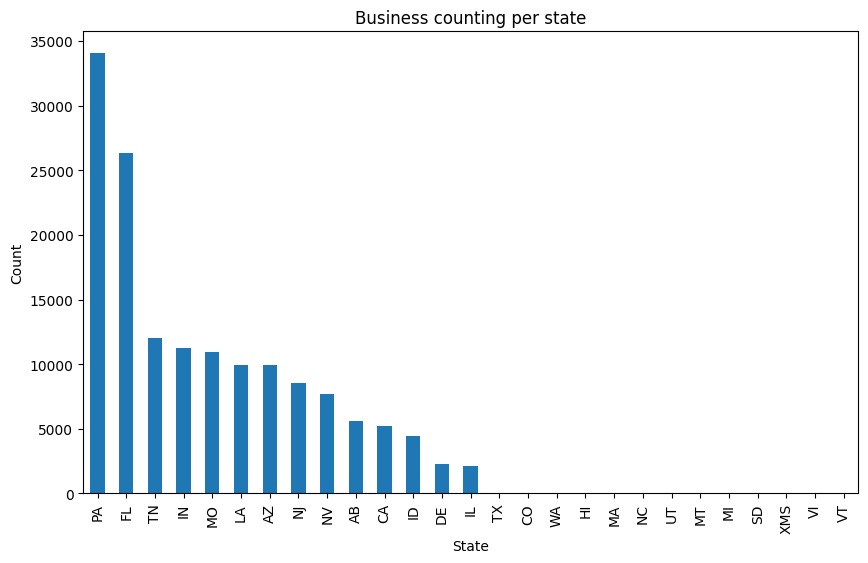
\includegraphics[scale=0.5]{../Images/dataexp.png}
\end{figure}
From the Figure \ref{fig:buscount} we can see that in "PA", we refer to Pennsylvania, a state located in the northeastern part of the United States. So I decided to conduct my analysis over the "PA" state due the amount of businesses present over there. Furthermore due the high dimension of the df it's difficult to create others type of graphics.
\section{Data Filtering}
As we discussed in the previous section \ref{sec:visdata} we want to targeting our recommender system in a specific area for a specific type of business. So I decided to take \textit{"PA"} as state and \textit{"Restaurant"} as type of business. Moreover I filtered the new dataframe called \texttt{restaurant\textunderscore df} with another parameter called \texttt{is\textunderscore open} that when is equal to 1 means that this business is actually a running business.
\begin{lstlisting}[language={Python},label={lst:filtdata},caption={Filtering Pyspark df}]
# Filtering data
restaurant_df = df_business_pandas[(df_business_pandas['state'] == state) & (df_business_pandas['is_open'] == 1) & df_business_pandas['categories'].str.contains(type_business)==True].reset_index()
\end{lstlisting}
Here an example of \texttt{restaurant\textunderscore df} printed:
\begin{table}[h]
\centering
\small
\resizebox{\textwidth}{!}{%
\begin{tabular}{llllllllll}
\hline
\multirow{2}{*}{index} & \multirow{2}{*}{address} & \multirow{2}{*}{attributes} & \multirow{2}{*}{business\_id} & \multirow{2}{*}{categories} & \multirow{2}{*}{city} & \multirow{2}{*}{is\_open} & \multirow{2}{*}{name} & \multirow{2}{*}{stars} & \multirow{2}{*}{state} \\
 & & & & & & & & & \\
\hline
3 & 935 Race St & (None, None, 'full\_bar', \{'touristy': False, '... & MTSW4McQd7CbVtyjqoe9mw & Restaurants, Food, Bubble Tea, Coffee \& Tea, B... & Philadelphia & 1 & St Honore Pastries & 4.0 & "PA" \\
\hline
\end{tabular}%
}
\caption{Example of a restaurant\_df's row}
\label{tab:rowrest}
\end{table}
Note that the attribute and category columns must be preprocessed before being used.
\section{Data preprocessing}
Lets start to analyze the attribute column. As we can see they are in this form:
\begin{lstlisting}[language={Python},label={lst:attritemex},caption={Attributes item example}]
Row(AcceptsInsurance=None, AgesAllowed=None, Alcohol="u'none'", Ambience=None, BYOB=None,..)
\end{lstlisting}
So we need a function that allow us to extract key-value pairs in a format understandable to Python. Here the snippet:
\begin{lstlisting}[language={Python},escapechar=|,label={lst:extractvalue},caption={Extracting key-value from attributes}]
# Function for extracting key-value from attributes
def extract_values(row):
    if row is None or row == "{}":
        return {}
    
    attributes = {}
    pattern = r"(\w+)\s*=\s*([^,]+)" |\label{line:re}|
    matches = re.findall(pattern, row)
    
    for key, value in matches:
        value = value.strip("'")
        attributes[key] = value
    
    return attributes
\end{lstlisting}
To achieve the result I used the regular expression. More specifically the line~\ref{line:re} defines a regular expression pattern.The pattern captures two groups:
\begin{itemize}
 \item the key (composed of one or more word characters \texttt{\textbackslash w$+$})
 \item the value (composed of one or more characters that are not a comma \texttt{\textbackslash $[\hat,]+$}), separated by an equal sign with optional whitespace around it.
 \end{itemize} 
Then we apply the function over all the rows of column attributes.
Now that the format seems to be good we proceed to create an entire \texttt{restaurant\textunderscore df\textunderscore attr} in which the attributes are extracted making a new column of the df and populating it with 0 or 1 based on their original value. An example are in the Table \ref{tab:restattrtable}.
\\
\begin{table}[]
\caption{Example of \texttt{restaurant\textunderscore df\textunderscore attr} elements} 
\label{tab:restattrtable}
\begin{tabular}{|l|l|l|l|l|l|}
\hline
BestNights & RestaurantsCounterService & WiFi & ... & Smoking & CoatCheck \\ \hline
0          & 1                         & 0    & ... & 0       & 0         \\ \hline
1          & 0                         & 1    & ... & 1       & 1         \\ \hline
\end{tabular}
\end{table}
We apply this reasoning also for categories obtaining the \texttt{df\textunderscore categories\textunderscore dm}. It will be useful to create the \texttt{df\textunderscore final}, a fundamental component for the recommender system. So in the Chapter \ref{ch:recsys} we are going to understand how recommendation systems work in theory.
\chapter{Recommender system}\label{ch:recsys}
\chapter{Creation of a Content-based Recommender system}\label{ch:recsyscontbased}
\chapter{Scalability and complexity}\label{ch:scalability}
\chapter{Results and experiments}\label{ch:results}
\chapter{Conclusion}\label{ch:conclusion}


\lstlistoflistings
\bibliographystyle{unsrt}
\bibliography{biblio}
\end{document}
